\setchapterpreamble[u]{\margintoc}
\chapter{Findings: Apps and their Artefacts}
%\julian{This chapter covers \uartefacts and \iartefacts. I'm currently revising this chapter based on Arosha's feedback in late July 2022. The underlying spreadsheet of the findings is \href{https://docs.google.com/spreadsheets/d/1PcwJ6E_X6peCP1dBPADEAJXOBpnb4JY1gSGNyPSxedA/edit?usp=sharing}{Mapping content to chapters} and you should have access from your Google account if you are helping me with this thesis.}

\begin{figure*}
    \centering
    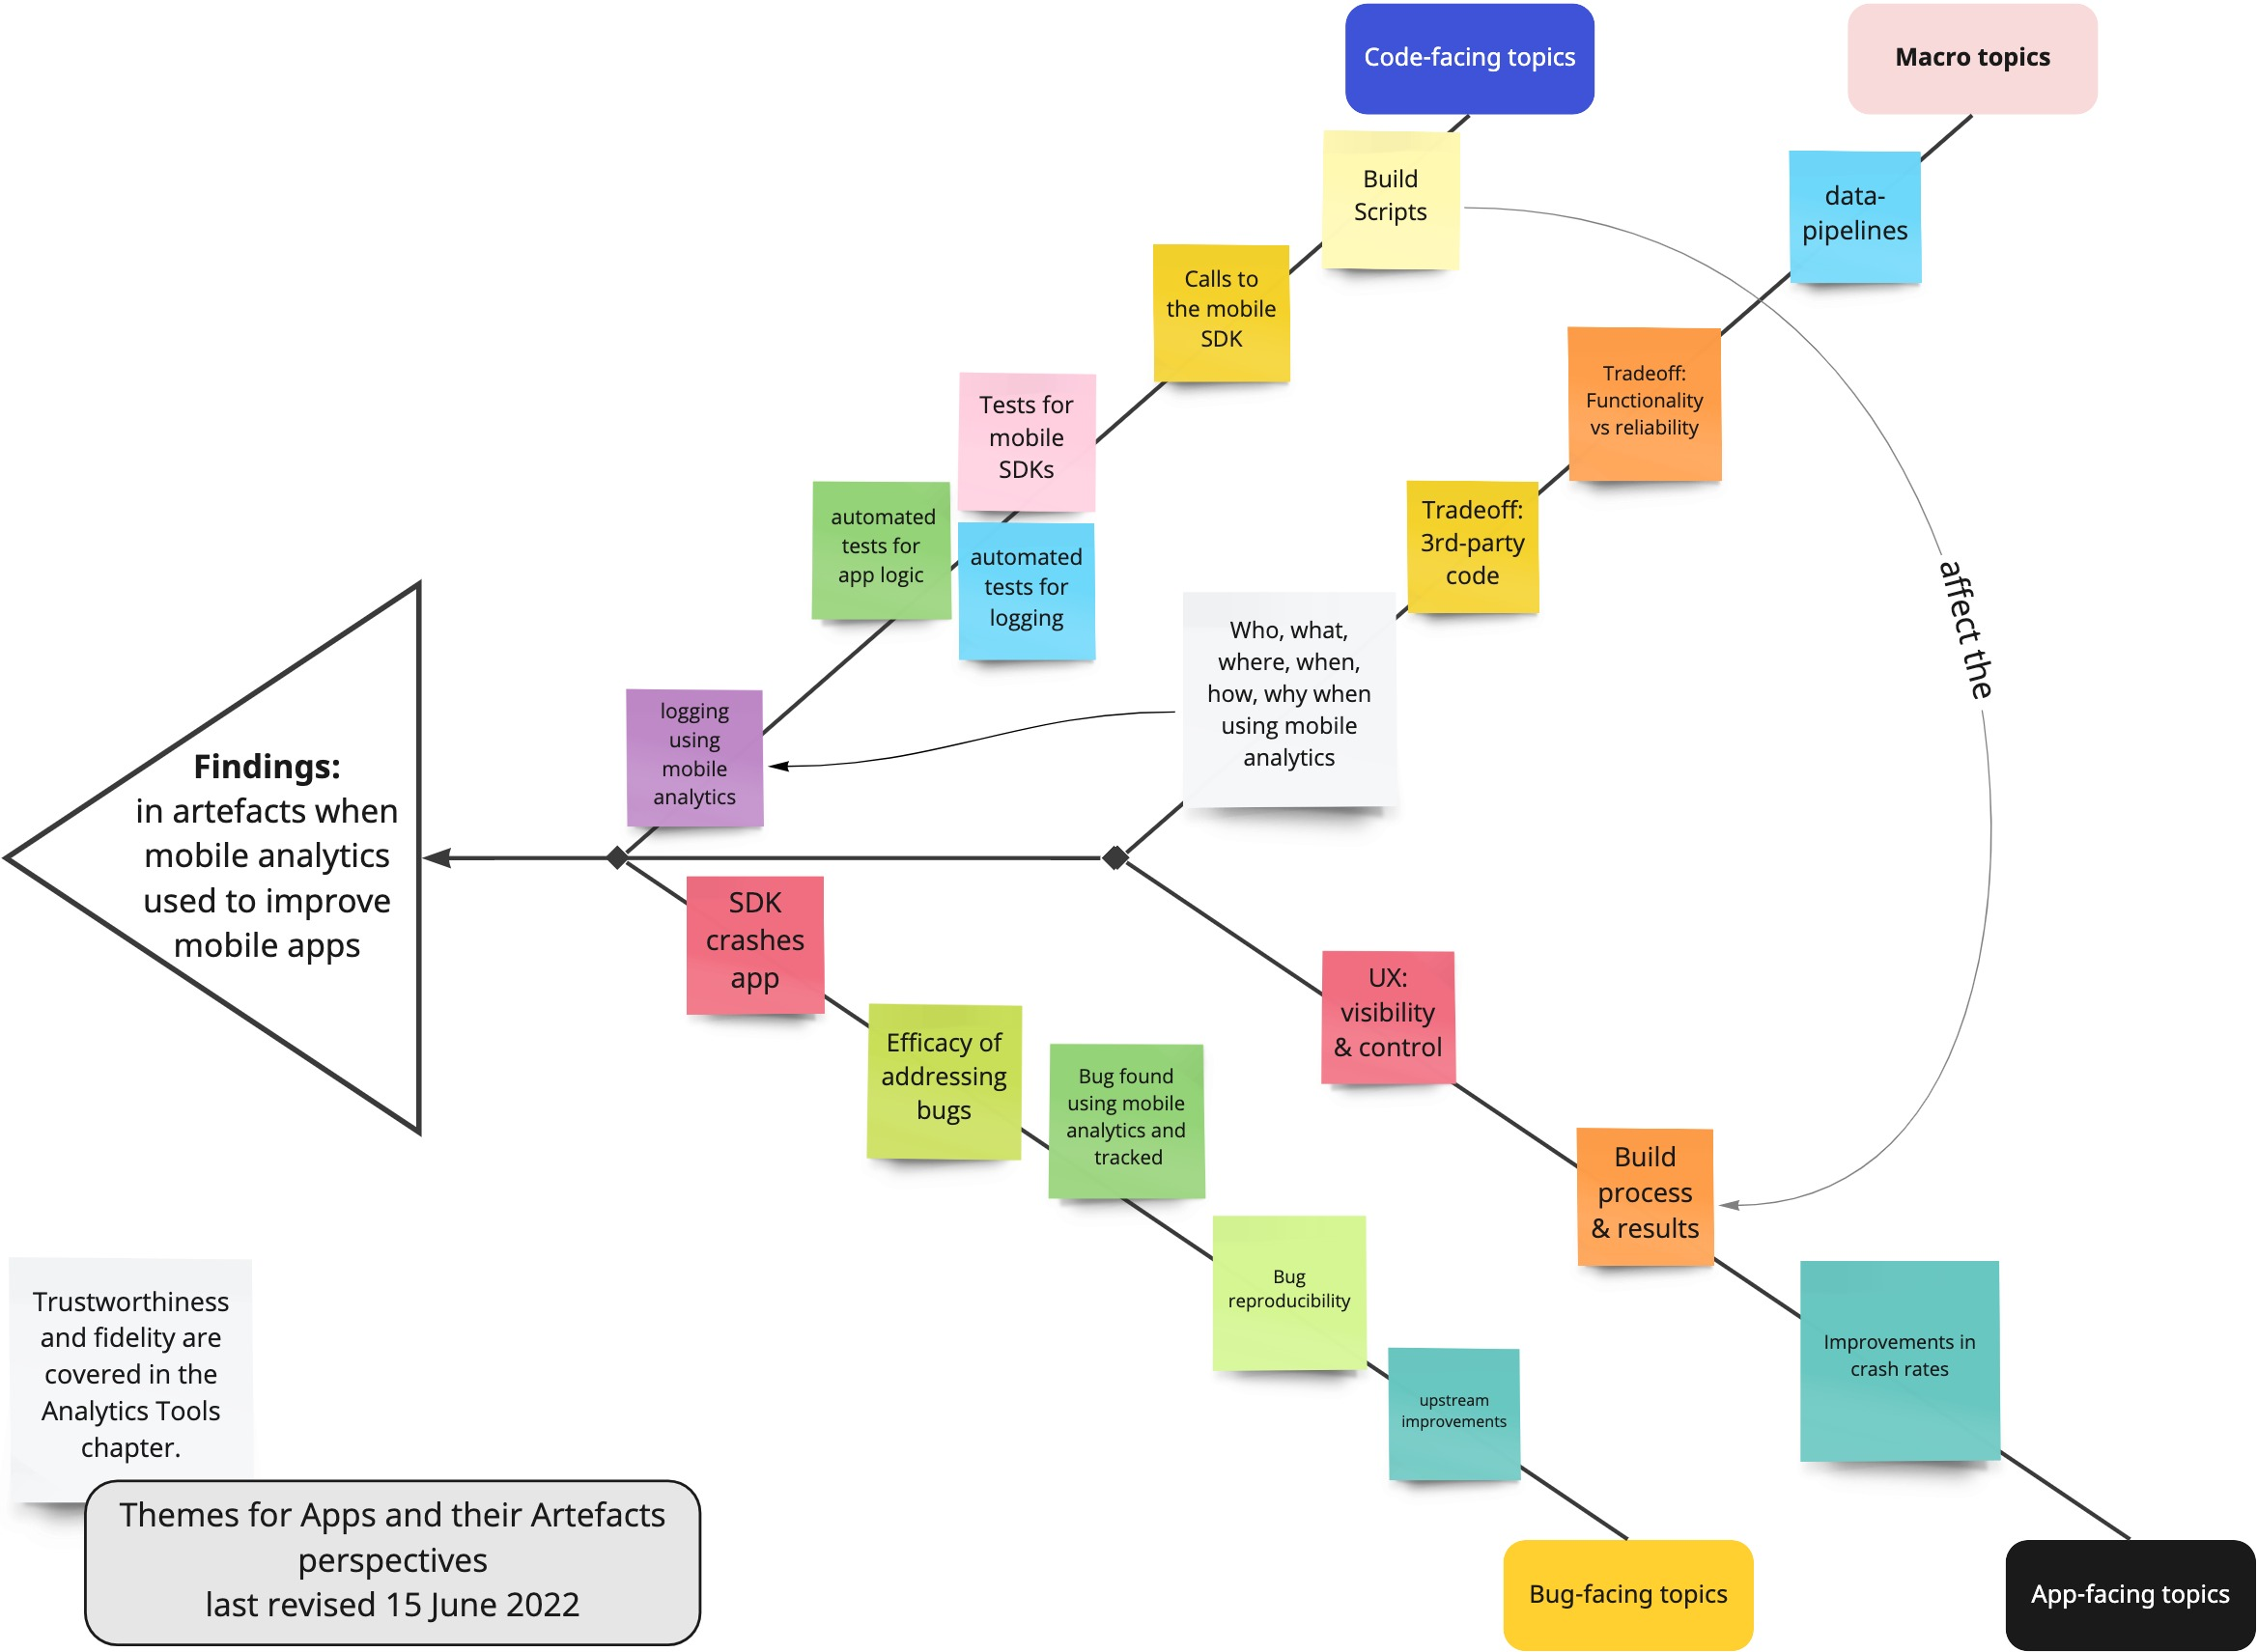
\includegraphics[width=0.8\linewidth]{images/rough-sketches/apps-and-their-artefacts-fishbone-15-jun-2022-d.jpeg}
    \caption[Apps and their artefacts fishbone diagram]{Apps and their artefacts fishbone diagram\\source: \href{https://miro.com/app/board/uXjVOts6mvo=/?share_link_id=402034254193}{diagram on miro.com}}
    \label{fig:apps-and-their-artefacts-fishbone}
\end{figure*}


This chapter presents the  findings for the research perspectives associated with apps and their artefacts, i.e. \uartefacts and \iartefacts. The artefacts associated with a mobile app development project are a product (or outcome) of developers' activity as they create and maintain the app. Beyond the obvious artefacts like the source code of the app, artefacts include items stored in the bug-tracking or issue management system of the project, as well as outputs from build processes, such as test results, the release binaries and outputs from mobile analytics.

Broadly, as shown in Figure \ref{fig:apps-and-their-artefacts-fishbone}, the mobile analytics topics that are relevant to app artefacts can be organised into themes based on their relationship to the code of the app, the bugs identified in the app and the app itself. Additionally, there are a set of broader topics relating to trade offs that developers need consider when including analytics in their app artefacts and managing the data pipelines associated with analytics.

This chapter presents the findings from the case studies together with exploration of grey data and literature, relating to each of these themes. This is followed by a discussion of how mobile analytics affects the artefacts associated with a mobile app project, drawing on the broader literature on how development teams use different types of artefact.

%The artefacts are a product, an outcome, of what developers do as they create and maintain their mobile apps. They include the source code of the codebase which evolves on an ongoing basis for active projects, any bug-tracking/bug-management system, outputs from builds including test results, outputs from mobile analytics. 

%To some extent the artefacts reflect macro (big-picture) topics including ethics, scaling, data-pipelines, engineering tradeoffs, and decisions on using third-party code. Figure \ref{fig:apps-and-their-artefacts-fishbone} illustrates the topics covered in this chapter.

\section{Code-facing topics}~\label{aata-code-facing-topics}
%\julian{This section needs reorganising to separate Crash and possibly Error reporting from the use of mobile analytics for other issues.}

The first broad category of themes relevant to the findings are associated with the artefacts of mobile app projects that are more closely connected to the code of the app. This includes 1) build scripts, 2) integration of the app with mobile analytics \Gls{sdk}s, 3) automated tests for the app, and 4) tests for mobile analytics \Gls{sdk}s. These are followed by introducing one of the ways app developers have used mobile analytics for remote logging.

\subsection{Build scripts}~\label{aata-build-scripts}
App developers use and maintain build scripts to build their apps and generally the build script combines with various build tools to customise the \gls{glossary-app-binary} (the code that's installed on app-centric mobile devices). Commonly used build variants include debug and release build targets. 
When apps include in-app mobile analytics often the build scripts are modified to specify the necessary SDK dependencies and the application's source code is modified to initialise the SDK. The documentation for Sentry's\index{Sentry} Android SDK provides a clear three step process of \textbf{Install}, \textbf{Configure}, \textbf{Verify}, so these are reproduced here~\footnote{Use permitted under their opensource license.}. Listing \ref{listing:build_gradle_for_sentry} is a typical example of how a mobile analytics dependency is added to the build file, this is Sentry's \textbf{install} step in their process.

\begin{listing}
\begin{minted}{groovy}
dependencies {
    implementation 'io.sentry:sentry-android:6.0.0'
}
\end{minted}
\caption[Install Sentry \texttt{build.gradle} to an Android app's codebase]{Example: Install Sentry \texttt{build.gradle} to an Android app's codebase\\source: \href{https://docs.sentry.io/platforms/android/}{Android Sentry Documentation}}
\label{listing:build_gradle_for_sentry}
\end{listing}

The \textbf{configuration} step requires a setting that is uniquely allocated by Sentry for this app when the developers use Sentry's online service. Listing \ref{listing:android_manifest_xml_for_sentry} shows the syntax of the configuration; the developers would need to obtain the unique dsn (data source name) to use for their app and use that value in place of the example value.

\begin{listing}
\begin{minted}[breaksymbol=, breakanywheresymbolpre=]{xml}
<application>
  <meta-data android:name="io.sentry.dsn"
  android:value="https://examplePublicKey@o0.ingest.sentry.io/0" />
</application>
\end{minted}
\caption[Configure Sentry for that Android app]{Example: Configure Sentry for that Android app\\source: \href{https://docs.sentry.io/platforms/android/}{Android Sentry Documentation}}
\label{listing:android_manifest_xml_for_sentry}
\end{listing}

\textbf{Verification} is not strictly part of the build scripts as it's part of the app, nonetheless it's included here since it is closely connected to the previous steps.

The code snippet in Listing \ref{listing:android_activity_to_verify_sentry_works_in_app} sends details of a caught exception to \myindex{Sentry}'s service each time the code is run. Running this code (by using the app) helps \textbf{verify} the installation and configuration steps have been completed adequately. Note: this code would generally be removed from the app once the verification has been completed successfully, developers would effectively replace it with custom code for any additional reporting not already provided automatically by the \Gls{sdk}. % https://docs.sentry.io/platforms/android/usage/  https://docs.sentry.io/platforms/android/enriching-events/breadcrumbs/  https://docs.sentry.io/platforms/android/configuration/integrations/okhttp/

During the period of this research, the SDKs have continued to evolve, with newer versions offering developers a greater range of information and also more automation of the underlying data collection.  For example the \myindex{Sentry} 3.1.0 Android Gradle plugin automatically instruments the \myindex{OkHttp} library if it's part of the app~\sidenote{\href{https://docs.sentry.io/platforms/android/configuration/integrations/okhttp/}{docs.sentry.io/platforms/android/ configuration/integrations/okhttp/}}.


\begin{listing}
\begin{minted}{kotlin}
import androidx.appcompat.app.AppCompatActivity
import android.os.Bundle
import io.sentry.Sentry

class MyActivity : AppCompatActivity() {
  override fun onCreate(savedInstanceState: Bundle?) {
    super.onCreate(savedInstanceState)
    try {
      throw Exception("This is a test.")
    } catch (e: Exception) {
      Sentry.captureException(e)
    }
  }
}
\end{minted}
\caption[Writing code to verify the install and configuration of the Android app]{Example: writing code to verify the install and configuration of the Android app\\ source: \href{https://docs.sentry.io/platforms/android/}{Android Sentry Documentation}}
\label{listing:android_activity_to_verify_sentry_works_in_app}
\end{listing}

The majority of the other SDKs used in the case studies offer equivalent installation, configuration, and verification steps and include developer-oriented documentation of these steps. However, it should be noted that they may use other terms to describe these steps.

\newthought{Build scripts encapsulate the build process}.  
At one extreme build scripts may fully automate multiple steps to the point of releasing a new version of an app in the app store. At the other extreme, many of the steps may be manual and performed unsystematically by the development team. Of course many projects are somewhere between these two poles, so they partly encapsulate the build process where humans have to perform the rest of the steps in the process. 

In the \myindex{Catrobat} case study, a mistake in a manual step of the build process meant the new release of the \myindex{Pocket Code} app did not include the correct information and stopped the in-app crash analytics from being reported. The Crashlytics SDK on Android needed two distinct keys, an API Key and a secret key~\footnote{StackOverflow has a good example of how a build script obtains these values from the environment in \href{https://stackoverflow.com/q/46814593/340175}{stackoverflow.com/q/46814593/340175}%~\cite{scott2017_android_app_crash_noclassdeffounderror_on_samsung_lollipop_devices}
. 
The relevant documentation is no longer available, it was at \href{https://docs.fabric.io/android/fabric/settings/working-in-teams.html}{docs.fabric.io/android/fabric/settings/working-in-teams.html} according to \href{https://stackoverflow.com/a/40667490/340175}{stackoverflow.com/a/40667490/340175}}, and presumably at least one of these was either missing completely or incorrect for that build.
% https://stackoverflow.com/questions/31596792/how-to-get-test-and-production-values-for-fabric-crashlytics 
% See also https://www.instabug.com/crashlytics-alternative 
% and a nice set of examples of how to integrate various SDKs including AppSee and Crashlytics in Ruby code https://github.com/HipByte/motion-fabric 

As an aside, in Grey Data, there is an excellent example not only of configuring the API Secret Key using the runtime environment (the method used by the Catrobat project) but of an adverse side-effect of changing the build target to a newer release of Android where the app then started to crash frequently on some Samsung device models~\sidecite{scott2017_android_app_crash_noclassdeffounderror_on_samsung_lollipop_devices}. 


\subsection{Calls to the Mobile Analytics SDK}
This research found and identified several distinct uses of mobile analytics by developers. Developers could apply none, any, or even all of these uses in their app for various in-app mobile analytics SDKs.

\begin{itemize}
    \item Instantiation only: a minimal integration that calls the SDK so that it is configured and runs in the background. No other calls are made to the SDK by the app, therefore the only analytics data is whatever is collected by default by the SDK.
    \item Reporting of caught exceptions (also known as Errors and/or error reporting). 
    \item Breadcrumbs: some SDKs provide a Breadcrumbs API, for others developers can implement and use custom events to generate an instance of a breadcrumb.
    \item Reporting of additional activities: for example screen and/or network activities. This may be performed automatically by the SDK or by developers writing API calls to do so.
    \item Remote logging using a mobile analytics SDK.
\end{itemize}

\newthought{Instantiation Only}
In joint research~\sidecite{harty2021_logging_practices_with_mobile_analytics} we discovered 50 of 107 active opensource Android apps only initialised the \myindex{Firebase Analytics} \Gls{sdk}. The other 57 made additional \Gls{api} calls to the \Gls{sdk}.

\newthought{Reporting caught exceptions} 
The Commercial project, \myindex{C1}, for example, made extensive use of Microsoft App Center to record caught exceptions, in particular, while \myindex{Moonpig} used \myindex{Firebase Analytics} for similar purposes. 

\newthought{Breadcrumbs}
\myindex{Moonpig} made extensive use of Firebase Analytics to record breadcrumb information to help determine and understand what led to undesirable events.  The commercial project, \myindex{C1}, used a proprietary distributed logging API for similar purposes. \myindex{LocalHalo} \emph{might} have logged similar data using \myindex{Flurry}, their business focused mobile analytics \Gls{sdk}. However, they did not appear to use \myindex{Sentry} to record breadcrumbs. 

Grey literature provides code examples and screenshots of creating custom code to add and subsequently use breadcrumbs to an Android app~\sidecite{daniel2019_breadcrumbs_to_enhance_your_crashlytics_experience}. 

\newthought{Reporting of additional activities}
Both \myindex{Moonpig} and \myindex{C1} made extensive use of mobile analytics to report additional activities. For \myindex{Pocket Code} some early, exploratory code was written to experiment with recording screens and activities however this work was abandoned with the realisation that Firebase was collecting and providing demographic and other potentially sensitive information from the project team's perspective. 

Logging, network IO, and mobile analytics combined in the industrial case study where a high crash rate in a new release was caused by a flawed implementation to increase the logging of network IO through the \myindex{OkHttp} library used by the Android app. 

Various mobile analytics \Glspl{sdk} automatically record activities and network I/O, a topic for the next chapter. 

\newthought{Mobile analytics for remote logging}
Some app developers also chose to use mobile analytics for logging, for example 57 active opensource Android projects available on github.com~\sidecite{harty2021_logging_practices_with_mobile_analytics}.

Mobile Analytics \Gls{sdk}s tend to use a network connection to transmit information from the end-user's device to central servers~\sidenote{I'm not aware of any exceptions nonetheless other transfer mechanisms are possible such as using memory cards or memory sticks.}. As an aside, it should be practical to write automated tests for mobile analytics \Gls{sdk}s to check the data the \Gls{sdk} emits. Doing so is outside the scope of this research and a possible topic for future research. % I have looked at PostHog's code which is actually based heavily on a fork of Segment's opensource code so I then also looked at some of Segment's Android code. I didn't find any code that actually checks the output or the transmission aspects. Note: https://segment.com/docs/connections/sources/catalog/libraries/mobile/android/ uses Square's Tape opensource library to persist event data. This might be something to explore adding memory-card/stick transfer to.

\begin{kaobox}[frametitle=Automated tests for logging]
While logging is rarely a \emph{source} of crashes in mobile apps it's often used: 
\begin{enumerate}[label=(\alph*)]
    \item  by the platform and/or the logging SDK record the actual crash and associated stack trace~\sidenote{Crashes can be read from an Android device using developer options and the adb command \texttt{adb logcat -b crash}.}, and
    \item by the app developers to record information to help the app developers diagnose possible reasons for the crash~\sidenote{As an aside, Google developers worked with app developers to add logging to help diagnose crashes for some older Android devices \href{https://github.com/google/filament/issues/2418}{github.com/google/filament/issues/2418}.}.
\end{enumerate}

\myindex{PostHog} uses a ShadowLog in their tests of logging \\ \href{https://github.com/PostHog/posthog-android/blob/master/posthog/src/test/java/com/posthog/android/LoggerTest.java}{github.com/PostHog/posthog-android/.../LoggerTest.java}

\medskip % Vertical whitespace to allow space for the side notes without them overwriting each other.

As mentioned in \secref{section-small-experimental-android-apps} as part of this research I co-wrote various small software projects to provide automated tests of local logging by Android apps~\sidecite{android_crash_dummy, android_log_assert}\index{GitHub Projects!Android Crash Dummy}\index{GitHub Projects!Android Log Assert}; these have been released under permissive opensource licenses.

\medskip % for consistency in the layout.

These projects may provide a basis to write automated tests for remote logging using mobile analytics.
\end{kaobox}


\subsection{Use of automated tests for the app}~\label{aata-use-of-automated-tests-for-the-app-topic}
Automated tests can dovetail with using mobile analytics to improve the reliability of mobile apps. For example, they can be used to demonstrate the reproducibility of crashes identified through mobile analytics. In the commercial case study this is what we did for various crashes reported via Android Vitals. For one of these an equivalent example has been released as an opensource project at \index{Kotlin} \href{https://github.com/julianharty/KotlinNPE}{github.com/julianharty/KotlinNPE} which tests the fix. This project is partnered by another opensource project \href{https://github.com/julianharty/AutomatedTestingWithKotlin}{github.com/julianharty/AutomatedTestingWithKotlin} as we wanted to find a way to run tests directly in a \gls{jvm} without needing the overhead of the Android runtime. When automated tests need the Android runtime the build process and the runtime environment become much more complicated and the elapsed runtime for the tests can take several orders of magnitude more time.

Use of automated tests for bug reproduction/bug fixes was patchy in all of the development teams in the case studies. \emph{I.e.} they all chose to `fix' at least some crashes directly without the support of automated tests. Their success rates of writing these fixes varied. For example the Kiwix developers were able to fix various NullPointerExceptions directly in the application's source code whereas they were not able to fix the crashes in the custom downloader code. 

\myindex{Moonpig}'s development team chose to write automated tests where they believed they would be helpful, for some of the failures they believed they had sufficiently detailed sources of information to apply some fixes directly to the codebase, in part through their extensive use of \myindex{Firebase Analytics} for in-app logging and usage monitoring.

% COULD_DO if it'd be useful - review the fixes applied after the PocketCode hackathon to see how many included automated tests. Then write up the results here.


\subsection{Tests for mobile analytics SDKs}
Several types of tests have been found for mobile analytics \Gls{sdk}s, the first type are tests developers implement to \textit{check the plumbing works i.e.} that the \Gls{sdk} has been integrated and configured adequately for a basic confidence test. The second type are written to check the \Gls{sdk} at a unit or module level.

\newthought{Support in the SDK: } 
All of the in-app crash reporting \Gls{sdk}s encountered during the research included confidence tests (verifying the \Gls{sdk} has been configured adequately). The app-centric case studies might have used these verification tests when they enabled their mobile analytics \Gls{sdk}s, however as noted earlier these verification tests are unlikely to be long-term additions to the app's codebase and no evidence is available on whether they were used or not. 

\newthought{Crash reporting tests: } 
The \myindex{Catrobat} project included automated unit tests for crash reporting~\sidenote{The source code for the tests is available online \href{https://github.com/Catrobat/Catroid/pull/2419/files}{github.com/Catrobat/Catroid/pull/2419/files} and the pertinent code review discussions are available online \href{https://github.com/Catrobat/Catroid/pull/2371}{github.com/Catrobat/Catroid/pull/2371}.} until the project removed \myindex{Firebase Analytics} from the project several months after the core case study~\sidenote{Pull request that removed the tests \href{https://github.com/Catrobat/Catroid/pull/3832}{github.com/Catrobat/Catroid/pull/3832}.}. \myindex{Kiwix} does not use in-app mobile analytics so does not have any tests for them either. None of the interview-led case studies provided details of whether they have crash reporting tests.

\newthought{Automated tests for the opensource SDKs: }
Automated tests for the opensource SDKs used in the app-centric case studies are available on github.com: \myindex{Amplitude} Android~\sidenote{\href{https://github.com/amplitude/Amplitude-Android/search?q=test}{github.com/amplitude/Amplitude-Android/search?q=test}}, \myindex{Segment}.io's Android SDK~\sidenote{ \href{https://github.com/segmentio/analytics-android/search?q=test}{github.com/segmentio/analytics-android/search?q=test}}, \myindex{Sentry}'s Android SDK~\sidenote{\href{https://github.com/getsentry/sentry-java/search?q=test}{github.com/getsentry/sentry-java/search?q=test}} and \myindex{React Native} SDK~\sidenote{\href{https://github.com/getsentry/sentry-react-native/search?q=test}{github.com/getsentry/sentry-react-native/search?q=test}}, and \myindex{Firebase}'s Android SDK~\sidenote{\href{https://github.com/firebase/firebase-android-sdk/search?q=test}{github.com/firebase/firebase-android-sdk/search?q=test}}, amongst others. 

While these SDKs have various automated unit tests, end-to-end tests for the SDKs are harder to find. Segment provides an End to End test  \href{https://github.com/segmentio/analytics-android/blob/master/analytics-samples/analytics-sample/src/androidTest/java/com/segment/analytics/E2ETest.java}{E2ETest.java}~\sidenote{They also provide a standalone command-line test tool \href{https://github.com/segmentio/library-e2e-tester}{github.com/segmentio/library-e2e-tester}.}, and clearly describe why they have chosen to test their service in production~\sidecite{segment2018_we_test_in_production_you_should_too}.  


\section{Bug-facing topics}~\label{aata-bug-facing-topics}
Mobile analytics SDKs are software development projects, and like other software they may have material flaws and some can even stop an app from working. 

\begin{itemize}
    \itemsep0em 
    \item SDK can cause the app to crash e.g. \href{https://github.com/segmentio/analytics-android/issues/732}{Crash during Google Pre-launch report \#732}.
    \item Some developers choose to record bugs for failures reported via mobile analytics. (e.g. Kiwix \href{https://github.com/kiwix/kiwix-android/issues/2482}{Kiwix Android Issue 2482:} for a Crash Report for an IllegalArgumentException in release 3.4.1 of the Kiwix Android app). Note: As part of reviewing this bug I noticed at least one new bug in Android Vitals, where they list the same crash cluster several times in the results, details are in the issue on GitHub.
    \item Bug reproducibility, including the use of automated tests.
    \item The efficacy of addressing bugs.
    \item Obviating some bugs by replacing Java code with \myindex{Kotlin} (Upstream improvements).
\end{itemize}

\newthought{Intermittent appearances of bugs}~\label{section-intermittent-appearances-of-bugs-55-crashes}
In some instances, failures have remained submerged for several releases. Mobile Analytics helps to surface (detect) these failures when they do appear. 
For instance with the \myindex{Kiwix} Android app, in September 2019 there were 55 crashes reported for a \texttt{WebViewFactory MissingWebViewPackageException}\index{WebView}; see Figure~\ref{fig:55-crashes-WebViewFactory-MissingWebViewPackageException}. This crash disappeared for several releases before reappearing. The disappearance might have been for various reasons, a possible reason was simply the particular user who was adversely affected stopped using the app. 

\begin{figure*}
    \centering
    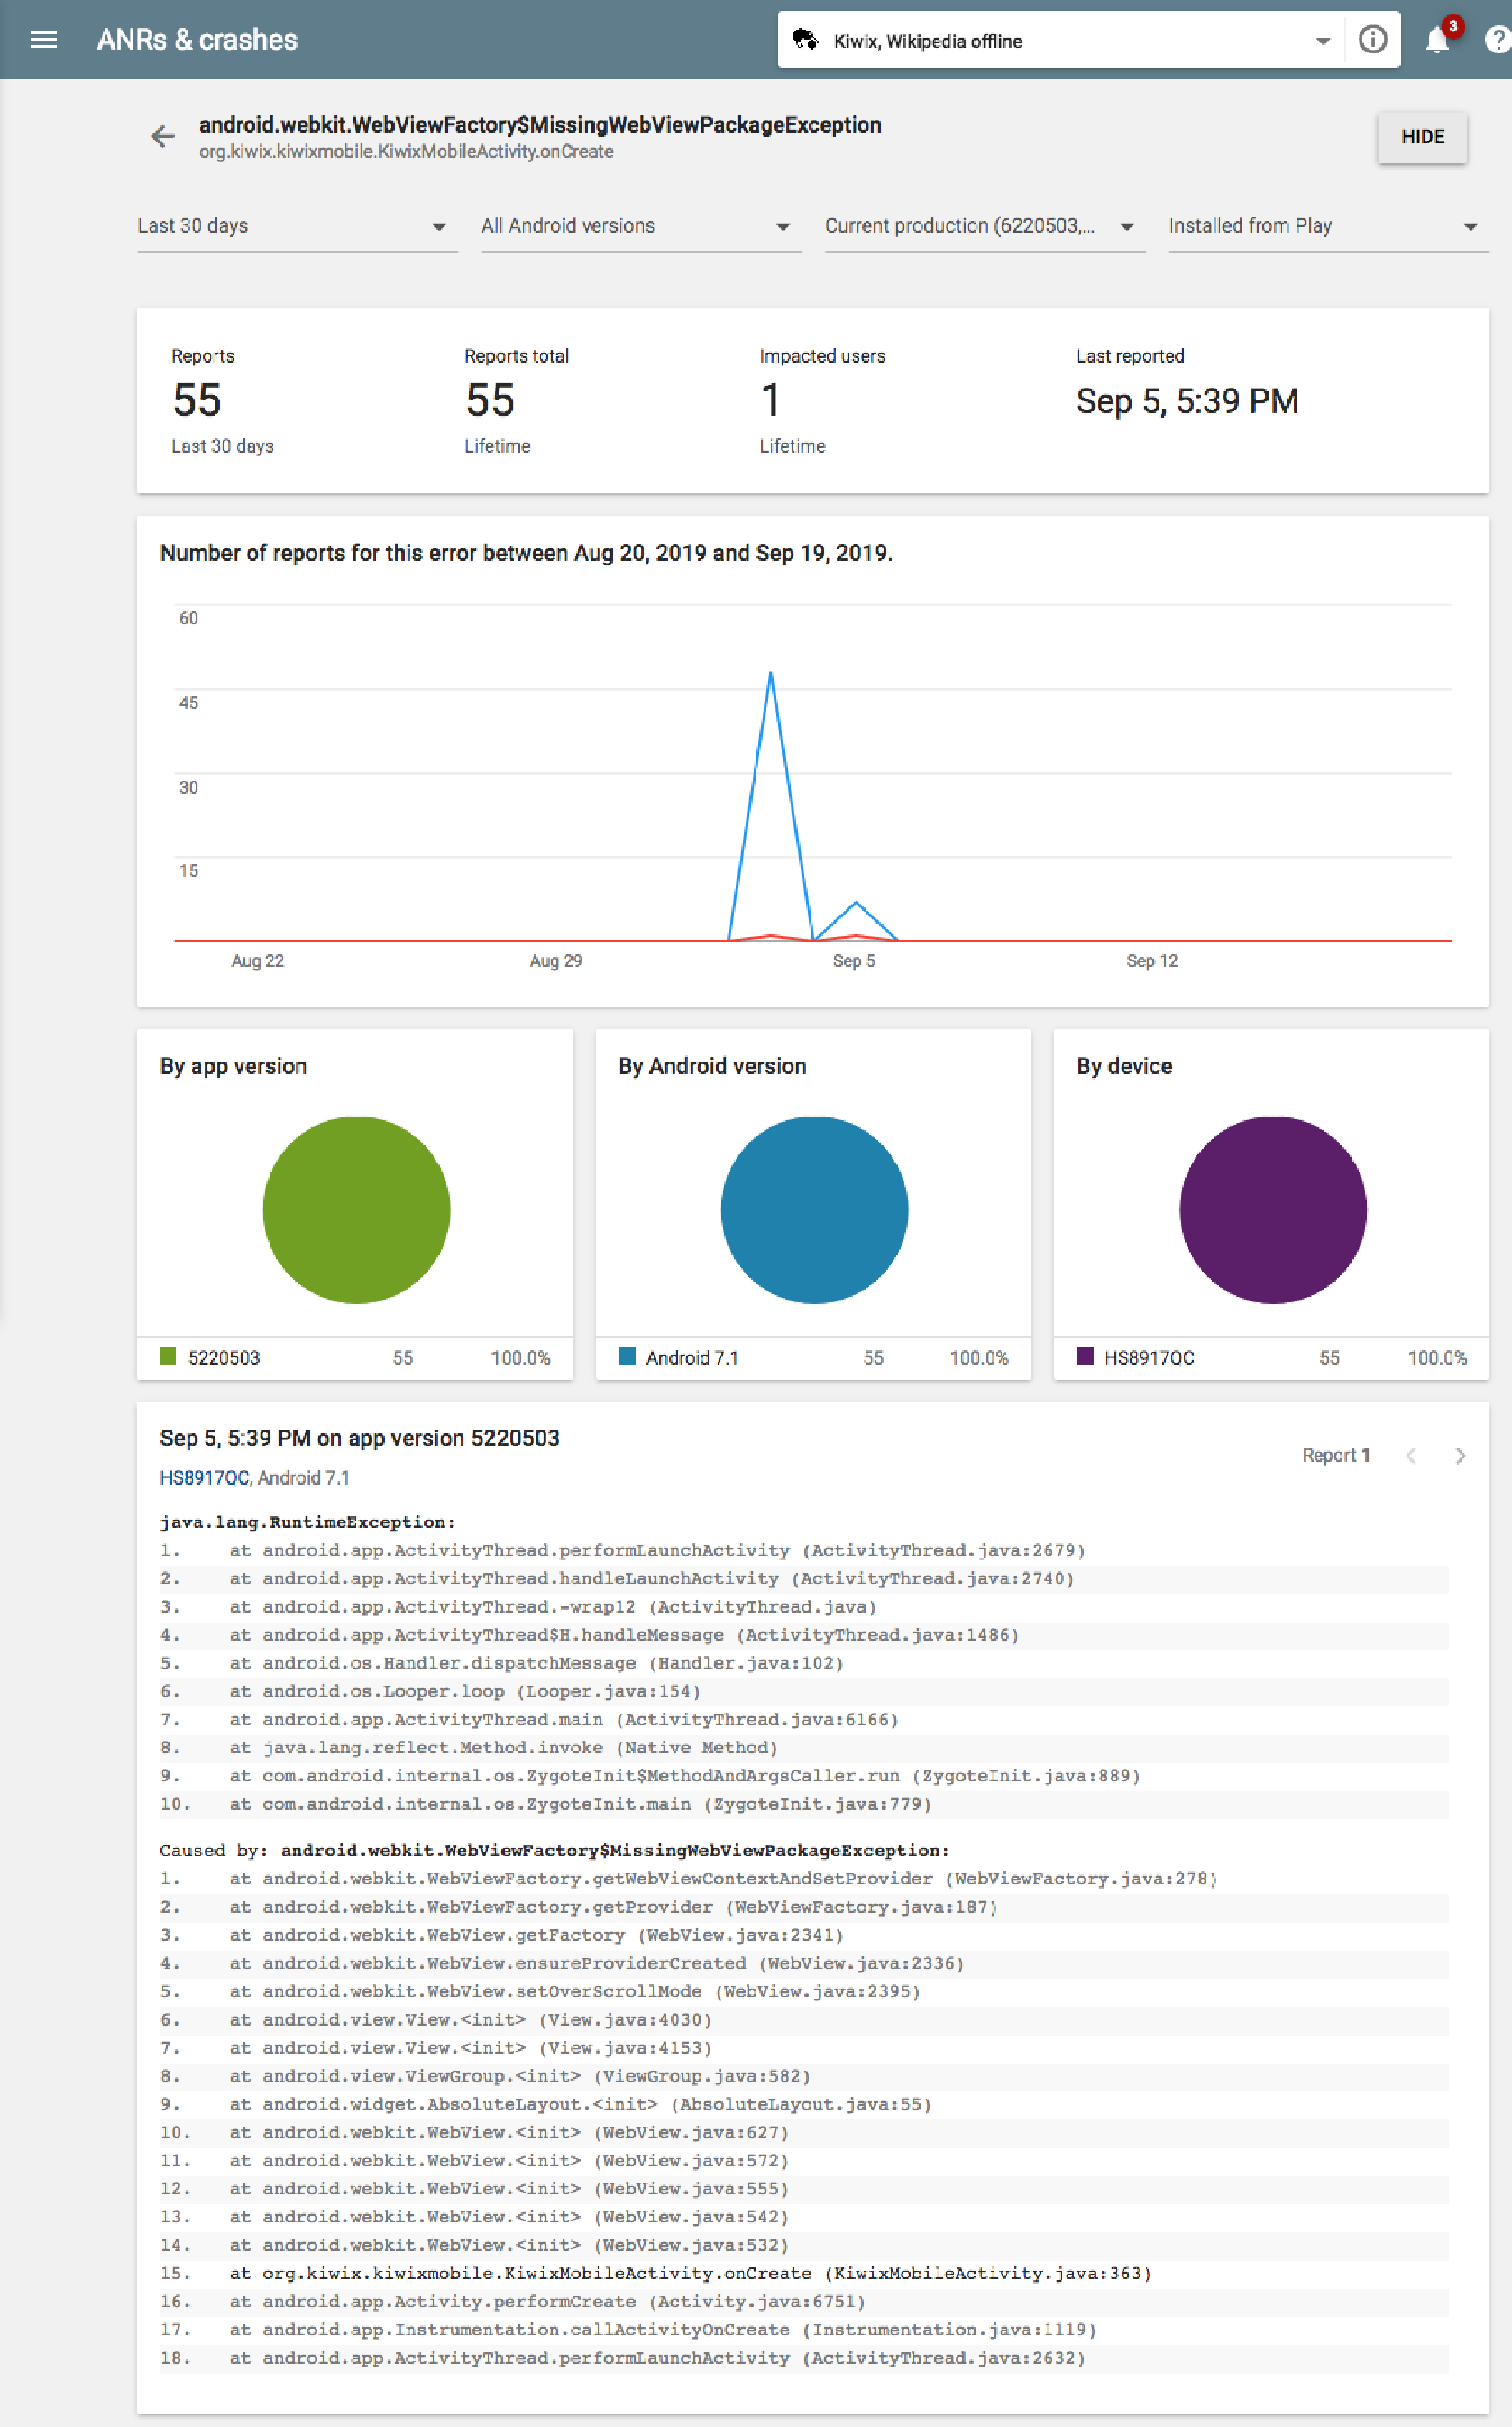
\includegraphics[width=0.9\linewidth]{images/android-vitals-screenshots/kiwix/55-crashes-WebViewFactory-MissingWebViewPackageException_2019-09-19-kiwix_trimmed.pdf}
    \caption{Kiwix Android 55 crashes for one user}
    \label{fig:55-crashes-WebViewFactory-MissingWebViewPackageException}
\end{figure*}

\FloatBarrier
\section{App-facing topics}~\label{aata-app-facing-topics}
Three topics in particular focus on the mobile app. The first of these is the most closely connected to the main research question (see \ref{overall-research-question}, on page \pageref{overall-research-question}), in terms of improvements to the product quality. 


\begin{itemize}
    \itemsep0em
    \item Improvements in crash and ANR rates.
    \item Build scripts can affect the behaviour of the app.
    \item User Experience of apps with in-app analytics (visibility and control aspects).
\end{itemize}

\subsection{Improvements in crash rates}~\label{aata-improvements-in-crash-rates-topic}
For both \myindex{Catrobat} and \myindex{Kiwix} the hackathon\index{Hackathon} and the post-hackathon bug fixes were highly effective in terms of cumulatively reducing the crash rate over several subsequent releases. % TODO Check whether the releases were contiguous.
The Catrobat case study replicated the improvements seen in the Kiwix case study and also the efficacy of using a hackathon as an immediate intervention. Note: the discussion chapter discuss limitations of hackathons and the useful half-life of hackathons in \secref{discussion-half-life-of-hackathons}. 


For \myindex{Pocket Code}, the improvements in the stability of the app were particularly encouraging as the project had already implemented many of `good' development practices. Figure \ref{fig:annotated_pocketcode_90_day_fabric_crashlytics_report} shows the cumulative improvement in the crash rate as measured by \myindex{Fabric Crashlytics}. Two releases to Pocket Code were made with fixes for issues identified during the hackathon\index{Hackathon}.

Note: Before the hackathon they had already addressed one of the worst offenders in terms of the crash rate and the effects of that improvement were rolling out during the weeks after the hackathon.
\sidenote{\href{https://jira.catrob.at/browse/CATROID-405}{JIRA issue 405}} was the \#1 issue with over 2000 crashes reported in the 30 days preceding the hackathon (and over 3200 in the lifetime of the app). However, it had already been addressed in JIRA issue 379\sidenote{``media download progress dialog crashers'' \href{https://jira.catrob.at/browse/CATROID-379}{jira.catrob.at/browse/CATROID-379}} and incorporated in to the most recent release \sidenote{Release:
0.9.65 Nov 13, 6:01 PM: Full rollout.} as part of a major effort to improve the code quality around the embedded WebView component.

Early indications are that the fixes related to the WebView have made a material improvement in the crash-rate for Pocket Code 2.45\% vs. 3.9.3\% on Monday \nth{18} November 2019; details are in Table \ref{tab:androidvitals_rollout_of_0_9_65}. Therefore, in terms of assessing any improvement that results from the work of the hackathon\index{Hackathon} the baseline is 2.45\%.

\begin{table}
    \centering
    \footnotesize
    \begin{tabular}{r|r|r|r}
        App version &Impacted sessions &Crash-free sessions &Number of sessions  \\
        \hline
        69 (0.9.65) &2.45\% &	97.55\% 	&~800 \\
        Production &&& \\
        \hline
        66 (0.9.64) &3.93\% &96.07\% 	&~3K
    \end{tabular}
    \caption{AndroidVitals: Improvement in crash-rate post WebView improvements}
    \label{tab:androidvitals_rollout_of_0_9_65}
\end{table}


\begin{figure*}
    \centering
    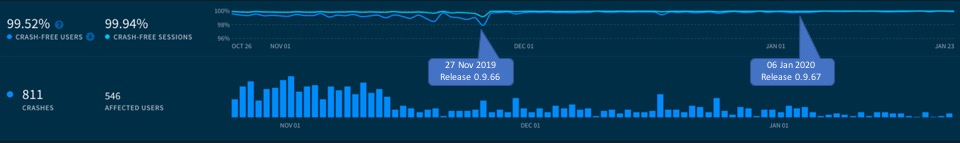
\includegraphics[width=\linewidth]{images/fabric-crashlytics/annotated_pocketcode_90_day_fabric_crashlytics_report.jpg}
    \caption{Fabric Crashlytics report on improvements in Pocket Code's crash rate}
    \label{fig:annotated_pocketcode_90_day_fabric_crashlytics_report}
\end{figure*}

\begin{table*}
    \centering
    \footnotesize
    \tabcolsep=0.06cm
    \begin{tabular}{r|r|r|r|r}
    \small
        App version &Impacted sessions &Crash-free sessions &Number of sessions &Period \\
        \hline
        72 (0.9.68) &1.26\% &   98.74\%     &~9K  &11-Jan-2020 to 08-Feb-2020 \\
        71 (0.9.67) &1.25\% &   98.17\%     &~14K &11-Jan-2020 to 08-Feb-2020 \\
        70 (0.9.66) &1.65\% &   98.35\%     &~5K  &04-Jan-2020 to 01-Feb-2020 \\
        69 (0.9.65) &2.05\% &	97.95\% 	&~2K  &22-Oct-2019 to 19-Nov-2019 \\
        \hline
        66 (0.9.64) &3.61\% &   96.39\% 	&~16K &22-Oct-2019 to 19-Nov-2019 \\
    \end{tabular}
    \caption{AndroidVitals: Improvement in crash-rate post Hackathon}
    \label{tab:androidvitals_crashrate_post_hackathon}
\end{table*}

Some notes on Table~\ref{tab:androidvitals_crashrate_post_hackathon}:
\begin{enumerate}
    \item The data was reported for thirty-day periods, one of three durations available in the user interface. All figures were calculated and provided by Google's Android Vitals analytics.
    \item The reports exclude small aggregate counts that fail to meet Google's reporting thresholds.
    \item The percentages fluctuate depending on where releases are in their maturity (their production lifecycle). Therefore these values are spot figures calculated that day and indicative rather than necessarily being suitable for calculating ratios for different periods. 
    \item These reports appear to be regenerated once a day, roughly 24 hours apart.
    \item It is unclear whether the underlying data is filtered to limit it to apps only installed by end users of production releases from Google Play.
\end{enumerate}


\begin{table*}
\caption{Reductions in Kiwix Crash Rates}
\footnotesize
\begin{center}
\begin{threeparttable}
\begin{tabular}{c c c c}
    \toprule
&\multicolumn{3}{c}{30-day crash rates reported in Android Vitals~\tnote{0}} \\
\midrule
\multirow{2}{*}{.} &\multicolumn{2}{c}{Kiwix Apps} \\
Stage &Release&\cellcolor[HTML]{efefef}Experiment &Control  \\

&\cellcolor[HTML]{efefef}&\cellcolor[HTML]{efefef}Kiwix & WikiMed English \\

1 &0 
  &\cellcolor[HTML]{efefef}5.07\% &1.13\% \\
2 &1 &\cellcolor[HTML]{efefef}3.12\%~\tnote{1} &\multirow{2}{*}{\cellcolor[HTML]{A8A8A8}}... \\
3 &2~\tnote{2} &\cellcolor[HTML]{efefef}1.59\%~\tnote{3} & \cellcolor[HTML]{A8A8A8}... \\
  &3 &\cellcolor[HTML]{efefef}0.53\%~\tnote{4} &1.09\%~\tnote{5} \\
4 &4 &\cellcolor[HTML]{efefef}0.72\%~\tnote{6} &0.60\%~\tnote{7} \\
  &4~\tnote{8} 
&\cellcolor[HTML]{efefef}0.55\% &0.41\% \\
  &5 &\cellcolor[HTML]{efefef}0.40\%~\tnote{9} &0.26\%~\tnote{10} \\
  \bottomrule
\end{tabular}
\begin{tablenotes}
  \item[0] Except when otherwise noted.
  \item[1] Kiwix Release 2.5 with the previous custom download facility replaced by a Google Android downloader.
  \item[2] The code is under 25 lines including 10 lines of comments~\url{https://github.com/kiwix/kiwix-android/pull/1388}.
  \item[3] Aggregate crash rate over 7 days for versions 2.4, 2.5.1, 2.5.2, 2.5.3 (to Aug \nth{26} 2019).
  \item[4] Previous 30 days crash rate, before release 3.1.2 pushed the crash rate up (same graph as TODO).
  \item[5] \emph{Unchanged release from the first control.}
  \item[6] Includes 3.1.2 which had an average (mean) crash rate of roughly 1.7\% (roughly \nth{31} Dec 2019).
  \item[7] A mixed set of crash rates, averaged by Android Vitals. For the first updated release of Wikimed (the 2019-12 release).
  \item[8] As usage increased of the more reliable releases the averages declined.
  \item[9] The crash rates for releases 3.2.1 are 0.23\% and 3.3.1 are 0.31\%
  \item[10] Release 2020-03 actually has a crash rate of around 0.05\% the numbers are higher as there are still significant volumes of usage on the previous 2 releases.
\end{tablenotes}
\end{threeparttable}
\end{center}
\label{tab:kiwix-evaluation-reductions-in-crash-rates}
\end{table*}
%%%% Isabel recommends creating a timeline instead - sounds good SHOULD-DO

Table~\ref{tab:kiwix-evaluation-reductions-in-crash-rates} provides a comparison of the crash rates for the experiment and the control apps over four stages of this case study. There were three phases that interleave with these four stages.

The stages are:
\begin{enumerate}
    \itemsep0em
    \item The baseline,
    \item Simplifying the most buggy code (which was the downloader),
    \item Applying the concepts in the research to the experiment,
    \item The new normal when mobile analytics is actively used.
\end{enumerate}

With the \myindex{C1} industrial case study the crash rate was reduced fourfold and the \Gls{anr} rate was reduced twofold.\sidenote{The actual values are confidential.} 
Furthermore, when a developer inadvertently introduced the exception that led to a short term crash rate of over 10\%, caused by a flaw logging \myindex{OkHttp} network responses, the project team were able to quickly detect and address the cause. One the updated release was rolled out the crash rate returned to approximately the previous mean value.  

\begin{figure}
    \centering
    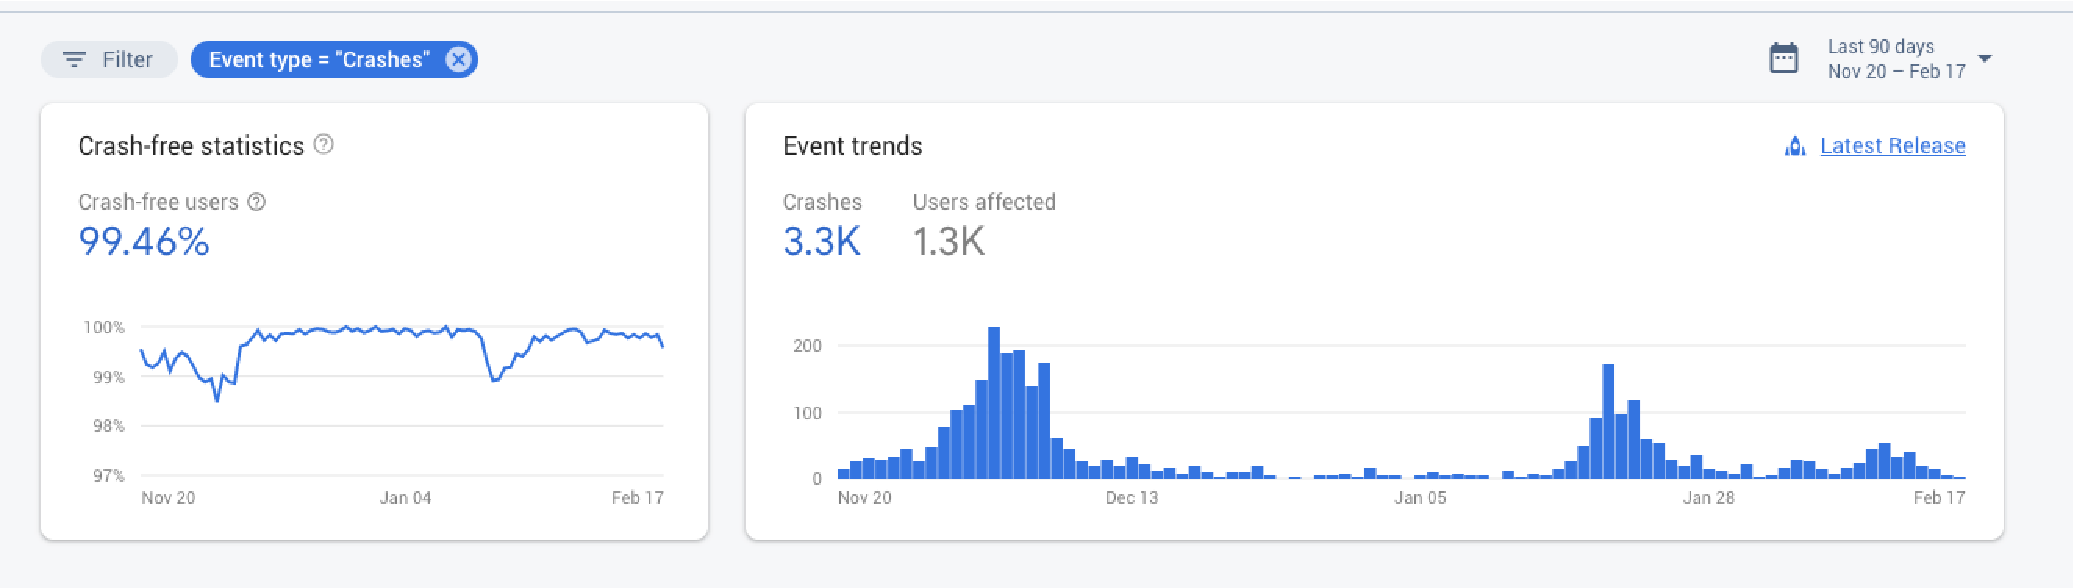
\includegraphics[width=\linewidth]{images/moonpig/firebase_crash_graph_90_days_feb_2020.pdf}
    \caption[Moonpig: Firebase Analytics illustrating two crashes that reached production]{Moonpig: Firebase Analytics illustrating two crashes that reached production before being addressed}
    \label{fig:moonpig-firebase-analytics-two-rogue-crashes}
\end{figure}

\myindex{Moonpig} provided various details of two crashes that emerged in production, including several graphs. Figure \ref{fig:moonpig-firebase-analytics-two-rogue-crashes} illustrates the effects of the crashes where they adversely affected the crash-free session scores and shows the restoration of higher reliability as each crash was addressed.


\subsection{Improvements in ANR rates}~\label{aata_improvements_in_anr_rates_topic}
Several of the case studies experienced bursts in the \Gls{anr} rates for at least one of the Android apps. These included \myindex{Catrobat}'s \myindex{Pocket Code} app, where 
\href{https://jira.catrob.at/browse/CATROID-411}{ANR at org.catrobat.catroid.stage.StageListener.takeScreenshot (StageListener.java:664)} was fixed three months after the hackathon and merged into v0.9.70 of Pocket Code in \href{https://github.com/Catrobat/Catroid/pull/3402}{github.com/Catrobat/Catroid/pull/3402}. and the Commercial project, \myindex{C1}, where the ANR rate in one release escalated to approximately 10\% in a rogue release before being reduced steadily to less than 0.4\%, partly by replacing an outdated version of an in-house library developed by another part of the organisation.

In grey material, a company valued at approximately 5 billion USD, \myindex{Bumble},~\sidenote{\href{https://companiesmarketcap.com/bumble/marketcap/}{companiesmarketcap.com/ bumble/marketcap/}}
achieved a six-fold reduction of \Glspl{anr}. They implemented hybrid approaches to scrape the content of reports from \myindex{Android Vitals}, this was - in essence - similar to our work on \myindex{Vitals Scraper} however they used  Selenium~\sidenote{A popular test automation framework for web applications.} rather than TypeScript, and Vitals Scraper obtained a wider range of data and the individual failure logs. They also wrote an in-house library that uses Android's \myindex{\texttt{getHistoricalProcessExitReasons}} and \sidecite{salomonbrys_github_anr_watchdog}~\sidecite{bumble_chameyev2020_how_we_achieved_a_6x_reduction_of_anrs_part1_collecting_data}.

They used a multi-faceted approach to reduce the \Glspl{anr}, described in~\sidecite{bumble_chameyev2020_how_we_achieved_a_6x_reduction_of_anrs_part2_fixing_anrs}. In short they used data, metrics and analytics to inform their development work and they were highly effective in achieving the desired reductions over a series of releases of their Android apps.

\subsection{Build scripts can affect the behaviour of the app}
A previous section \secref{aata-build-scripts} explained how build scripts encapsulate the build process and how it's possible to adversely affect the behaviour of in-app mobile analytics. And in \secref{aiu-choosing-mobile-analytics-topic} of the previous chapter, how developers can choose to vary the behaviours of an app, \emph{e.g.} to increase the logging in debug builds. (In Android they can use `build variants' and `product flavors' to do so~\sidecite{android_build_variants_and_product_flavors}.)

Often developers wish to optimise the application binary to remove non-essential code and to obfuscate the object code within the binary to protect the intellectual property contained within. Both the optimisation and any obfuscation tend to occur for release (production) builds of an app, these may affect the behaviour of the app in ways end-users are hard-pressed to discern. When using in-app mobile analytics it's important to preserve this functionality in release builds. Some projects disable mobile analytics in debug builds and others, including case-study \myindex{C1}, use a distinct identifier to separate the traffic so they can be reported-on and analysed separately. (This is discussed by a Google engineer and an app developer in \sidecite{firebasegooglegroup2016_best_way_to_setup_release_debug_firebase_environment}.)


\subsection{User Experience of apps with in-app analytics}
The visibility of any end-user `agreement' varied across the apps in the app-centric case studies that used in-app mobile analytics. Most did not present users with this information, with the exception of \myindex{Pocket Code}.

It required end-users to read and agree to a lengthy legal agreement the first time they used the app. 

In contrast \myindex{Moodspace} took a light-hearted approach in their app, as follows: 

\begin{kaobox}[frametitle=Moodspace privacy policy]
``To make the app work well at all we collect the following anonymous data:
\begin{itemize}
    \item Crash reports: If you've never seen the app crashing, it's because as soon as one happens, we get a crash report. A little red light flashes in our office, a loud siren blares, and we release a fix right away. It's quite annoying actually.
    \item Analytics: We assume you're going to use the app a certain way. We're almost always wrong, and you often surprise us. Analytics lets us see how people like you actually use the app, so we can make improvements to the right places. Analytics can use the Google Advertising ID to identify you. This doesn't tell us anything about you (it's just some numbers and letters), but if you really want to trick us you can reset your Google Advertising ID at any time. Go to your device Settings > Google > Ads.''
\end{itemize}~\sidecite{moodspace2021_privacy_policy}
\end{kaobox}

None of the apps provided end-users with any mechanism to disable in-app mobile analytics.

\section{Macro topics}~\label{aata-macro-topics}
Macro-topics touch on multiple aspects of developing mobile apps. This research identified the following groupings of macro-topics:

\begin{itemize}
    \item Three of these have a common trait of \textbf{tradeoffs}\index{Tradeoffs} developers face, in ethics, in the use of third-party code, and in functionality.
    \item Two have a common trait of \textbf{scaling}\index{Scaling}: scaling use of mobile analytics by developers and within their engineering microcosm.
    \item Two cover the trustworthiness and fidelity of the mobile analytics as reflected in the artefacts.\emph{I have an inkling this material is better placed elsewhere in my thesis than this chapter. TBD.} 
\end{itemize}

\subsection{Tradeoffs}~\label{aata-tradeoffs-topic}
At least three types of tradeoffs were evident in the artefacts: 
\begin{enumerate}
    \item \textbf{Ethical tradeoff: } the effects of ethical decisions by the project team (covered in \secref{aiu-ethics-and-pii-topics},
    \item \textbf{Functionality tradeoff :} downgrading functionality to obtain reliability,
    \item \textbf{Third-party tradeoff :} use of third-party vs locally developed functionality.
\end{enumerate}

\newthought{Ethical tradeoffs :} (Tradeoff 1).
The clearest example from the case studies, as described in the previous chapter in \secref{aiu-ethics-and-pii-topics}, is where the \myindex{Catrobat} project chose to remove in-app analytics from \myindex{Pocket Code} to prevent data being collected by Firebase Analytics \emph{via this app} as other apps on the end user's devices almost certainly are using Firebase Analytics and reporting much or all of the demographic and geographic data to Google's systems.

\newthought{Reliability trumps enhanced functionality: } 
The core \myindex{Kiwix} Android app included a custom file downloader that downloaded material such as Wikipedia in German for offline use. This downloader kept track of partial downloads and also allowed end users to control when to allow the downloads and when to pause or stop them. This functionality was designed to help users often in areas with intermittent, controlled, and sometimes expensive connectivity to increase their chances of being able to download the content within their budget. To provide some concrete examples in some parts of the world users would download content that took several entire \emph{days} even if the connection didn't fail, and the cost of the connection was metered and capped to 1GB of data.

However, the code for the downloader had various bugs and flaws including several that caused the app to crash. These crashes meant the app had an excessively high crash rate in the Google Play App Store. The then lead developer for the Android codebase had not been able to tame the high crash rate. A consultant was hired who had worked on multiple other Android projects and codebases. This consultant proposed scrapping the custom downloader and replacing it with standard Android functionality provided by Google as part of the Android SDK. This proposal was accepted and implemented\sidenote{The Pull Request with the major changes is \href{https://github.com/kiwix/kiwix-android/pull/1170}{2.5 downloader \#1170}.} and it had the desired effect of reducing the crash rate of the core Kiwix Android app significantly, as illustrated in Figure \ref{fig:kiwix-crash-rate-drops-with-v2_5}. The headline reduction in the report is from 4.59\% to 3.12\% however this includes the interim period when the reduction was taking effect as more users received/installed the newer release, so the improvement was better than than this report suggests - roughly a reduction from over 4\% to 2\%. (The gap in the graph is one of the flaws discussed in the tools chapter, in \secref{tata-flaws-topic}.)

\begin{figure}
    \centering
    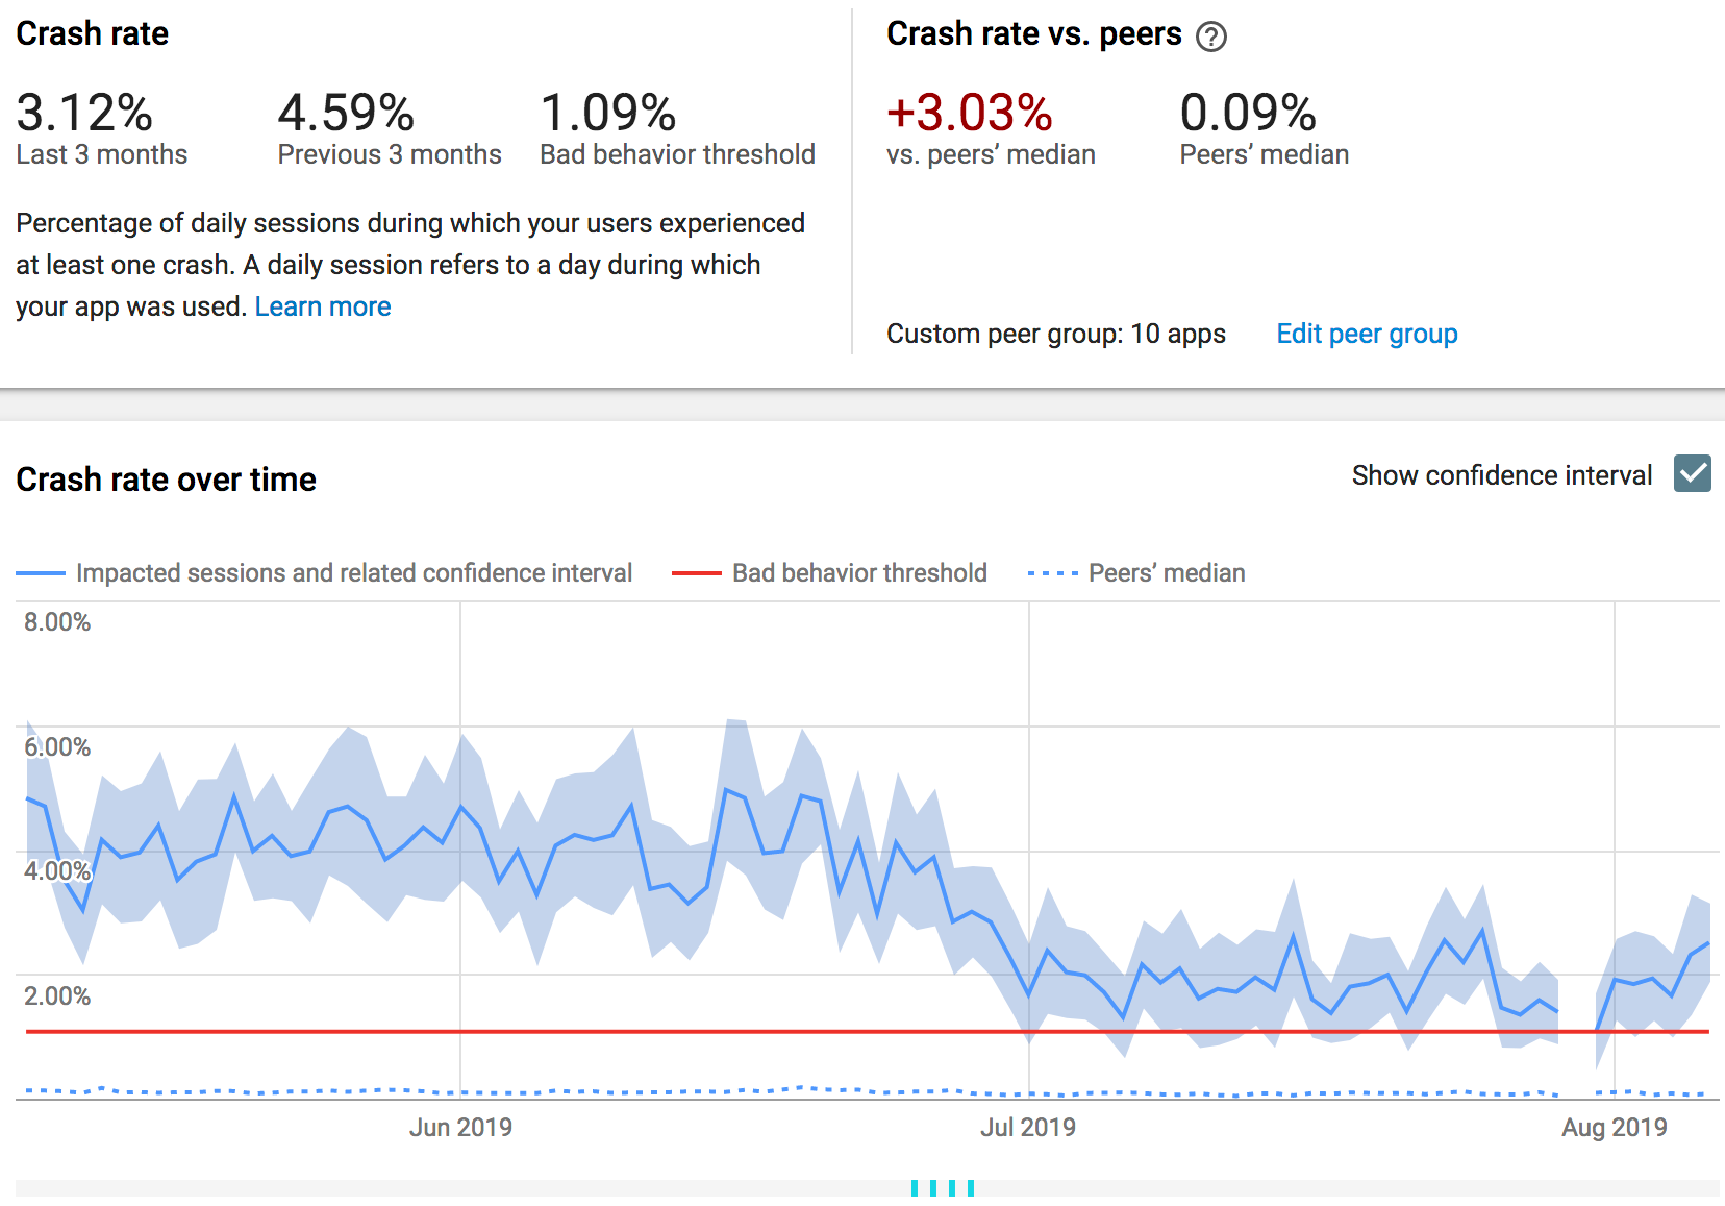
\includegraphics[width=\linewidth]{images/android-vitals-screenshots/kiwix/kiwix-crash-rate-drops-with-v2_5.pdf}
    \caption{Kiwix crash rate drops once custom networking code replaced}
    \label{fig:kiwix-crash-rate-drops-with-v2_5}
\end{figure}

However the standard Android downloader didn't provide equivalent facilities to continue partial downloads, or to pause and resume downloads, nor did it provide progress tracking information. Furthermore as the project team had chosen not to incorporate in-app mobile analytics the project team cannot easily determine the effects of these changes \emph{on the end users}. Bugs continue to surface occasionally on the project's GitHub site~\sidenote{\textit{e.g.} \href{https://github.com/kiwix/kiwix-android/issues/2845}{github.com/kiwix/kiwix-android/issues/2845}.} and users sometimes complain in reviews submitted to Google Play. Here are four \emph{verbatim} examples extracted from the developer's view of Google Play; (the developer's view has greater visibility into ratings and reviews than the public (user-oriented) view):

{\small
\begin{itemize}
    \itemsep0em
    \item ``\textit{Wikipedia nopic without images works again in version 11.18 with search function.! Top Unfortunately, now in March 21 again problems with wikipedia text with 14.2 gb. After 3/4 of the download the process breaks off every time! Too bad. Wikis with smaller amounts of data can be downloaded without any problems. Handling of the app very well.}'', Mar 22, 2021 % https://play.google.com/console/u/0/developers/9116215767541857492/app/4975184706939091905/user-feedback/review-details?reviewId=gp%3AAOqpTOGjPB5Em_o1TfLCzltkR7jvVhdVJAvBZlj9Y0-5i9FOcDaJ4Yjh1yqIHV5-qo-9HkbvGJSAHweXJOQodfo&corpus=PUBLIC_REVIEWS
    \item ``\textit{Download started and it could never finish}'', Mar 25, 2021 % https://play.google.com/console/u/0/developers/9116215767541857492/app/4975184706939091905/user-feedback/review-details?reviewId=gp%3AAOqpTOErPflFJDpyqiz4m4CJW3IPjYoXKGrO0SLZ4L94DwUPj662lAWuS0MOWAXfANZ2D6Vf--EkJLe1RPIeSqk&corpus=PUBLIC_REVIEWS
    \item ``\textit{Seems that library download is b0rken atm?}'', Oct 7, 2021 % https://play.google.com/console/u/0/developers/9116215767541857492/app/4975184706939091905/user-feedback/review-details?reviewId=gp%3AAOqpTOGVOb-MNO3ehakCJsUi7Ur-R_6QJkdnWzFDl7xh6KA28ZUATGKmBO7JzDTgPvULR0UhivkWMp2B0d83qpA&corpus=PUBLIC_REVIEWS
    \item ``\textit{Cant continue interrupted download}'', Oct 15, 2021 % https://play.google.com/console/u/0/developers/9116215767541857492/app/4975184706939091905/user-feedback/review-details?reviewId=gp%3AAOqpTOFxVKQVzPIrgcWHmCX8QnQXaqVkI8JFVwBzLYiDHJrdBbokV8SBDfRRjYltEqBp8lsLVTNFlix3fzFMHYA&corpus=PUBLIC_REVIEWS
\end{itemize}
}

And another review asks for the download manager that, ironically, used to exist (presumably without realising the app used to have one): ``\textit{edit: still there is no download manager. It is not possible to download the large files. Despite 100 megabits per second, I did not manage to load the large Wikipedia with images. The app itself is very good. Only the download of the huge files always breaks off. I load via PC. A download manager would not be bad.}'', Mar 12, 2021 % https://play.google.com/console/u/0/developers/9116215767541857492/app/4975184706939091905/user-feedback/review-details?reviewId=gp%3AAOqpTOEH9rOv2WWhAUTEChRwgT1Mrq5rYxEp9cQzrqjGDg6aeOccjVgxJeNFU_syr1wNPh9UMw71FKfM13iNy8k&corpus=PUBLIC_REVIEWS 

\newthought{Third-party code}: 
The third tradeoff is between third-party and locally developed code which generalises the second tradeoff found in the research (of trading functionality for reliability). As a concrete example, the \Gls{glossary-webview}\index{WebView}\Gls{glossary-webview}\index{WebView} component is ubiquitous on Android and found in many Android apps including several of those in the case study. %Is it worth the investment to find out how many of the apps use the Android WebView?. 

% Google's overview on the WebView component is available at https://developer.android.com/guide/webapps and https://developer.android.com/guide/webapps/webview-privacy discusses crash reporting and other data collection topics pertaining to apps using WebViews.

As projects, including the Kiwix team, discovered crashes can be reported in Android Vitals for the \Gls{glossary-webview}\index{WebView} component. These adversely affect the app's reliability as measured by Android Vitals. While the app developers can fix at least some of the causes of third-party components, including the \Gls{glossary-webview}\index{WebView} component, others may be beyond their direct control.

In March 2021, major apps including apps from the Amazon, BBC, Facebook, Google, Microsoft, etc. failed in use by a release of the \Gls{glossary-webview}\index{WebView} component~\sidecite{peters2021_google_fixes_issue_causing_android_apps_to_crash_etc_webview, bbcnews2021_google_fixes_crashing_android_app_issues, bbc_iplayer_app_april_2021_webview_information}. and Samsung's deadpan observation:

\begin{quote}
    ``If you are having an issue with the apps forcibly closing on your device, please follow the steps to resolve the issue. This problem has been resolved with the latest app updates of Android System Webview and Chrome, 89.0.4389.105 version.''

    ``To ensure that your apps do not crash, please update both Google Chrome and Android System Webview.''~\sidenote{Source: \href{https://www.samsung.com/ph/support/mobile-devices/google-webview-issue/}{www.samsung.com/ph/support/mobile-devices/google-webview-issue/}}
\end{quote}


All their respective app developers relied on a third-party software component developed and maintained by Google as part of Android. Furthermore, app developers who have incorporated the \Gls{glossary-webview}\index{WebView}\Gls{glossary-webview}\index{WebView} into their app sometimes introduced bugs in their use of the \Gls{glossary-webview}\index{WebView}\Gls{glossary-webview}\index{WebView}. Across a population of 146 opensource Android apps 124 WebView related bugs were found and the root causes analysed~\sidecite[][pp. 704 - 706]{hu2018_a_tale_of_two_cities_how_webview_introduces_bugs_to_android_applications}. Of these bugs, 15 introduced crashes~\sidecite[][p. 706]{hu2018_a_tale_of_two_cities_how_webview_introduces_bugs_to_android_applications}.

As Google Android notes online \url{https://developer.android.com/guide/webapps} there are various alternatives to using a \Gls{glossary-webview}\index{WebView}. They don't mention either a) developers developing their own user interface, or b) other third-party alternatives to their WebView (\emph{e.g.} \href{https://mozilla.github.io/geckoview/}{Mozilla's GeckoView}). 
% https://stackoverflow.com/questions/35559467/webview-alternatives (the answer is too dated to include in my thesis). and https://www.i-programmer.info/news/193-android/12900-the-geckoview-alternative-to-webview.html 
% https://android.gadgethacks.com/how-to/ditch-googles-webview-switch-androids-system-browser-bromite-0384227/ 

There is no silver bullet for developers in terms of choosing whether to write their own code or use third-party code. A \textbf{functionality tradeoff} (tradeoff 2) enabled the Kiwix team to improve the reliability at the cost of losing functionality where they replaced their own code with third-party code. 

The \textbf{third-party tradeoff} (tradeoff 3) allows developers to short-circuit the work of developing their own functionality at the risk of being unable to address some of the failures and problems related to using those third-party components. Examples from the app-centric case studies include the use of \myindex{RoboSpice} by \myindex{Moonpig}, and the \myindex{Expo framework} by \myindex{LocalHalo}.

\subsection{Scaling the use of analytics}
This topic presents two forms of scaling. The first is scaling-out the use of mobile analytics to more team members. The second is scaling up through the integration of mobile analytics where the data can be analysed at scale and combined with other large-volume data sources.

\newthought{Developers' access to, and use of, mobile analytics services: } %\improvement{From Isabel: reminds of the problems I raised in "Stuck in Limbo" security and other permissions preventing people using the tools they need. I'm also struck by the points about free versus paid for software - I think that's worth drawing out more - one of my interviewees talked about managers making decisions to save money by using free stuff/self building tools - but actually losing money/time because people are building tools rather than doing their work...}: 
In hindsight it may be blindingly obvious that in order to use mobile analytics one first needs access to the mobile analytics service and then to gain the habits and understanding to actually use what's been made available. And yet, in the majority of the case studies only a minority of the team leaders actually provided access to the majority of their team members. Examples of these case studies include LocalHalo where the CTO appeared to be the only developer with access to Sentry; in the Kiwix Android team where lead developers were the majority of those who had direct access to Android Vitals and similarly for the \myindex{Catrobat} project access tended to be for senior developers who were long-time team members\sidenote{Note: hard data was hard to obtain given the nature of the access granted to the researcher and discussions with the projects seldom led to the data being made available.}.

In the commercial project there were challenges in determining who granted access and subsequently developers had to obtain prior approval from their manager before requesting access to mobile analytics, and new team members were not necessarily even aware of the mobile analytics services so couldn't begin to request access. 

The clear counterexample was Moonpig where the development team members were routinely provided access to the mobile analytics as part of joining the development team. Furthermore the developers rotated on-duty to actively monitor the mobile analytics to find and respond to any anomalies; therefore they were encouraged to learn how to use, understand, and act on the reports in the mobile analytics services.

When copies of pertinent information, extracted from mobile analytics reports, are incorporated in to an issue tracking system they: a) are preserved generally for further use, and b) help to share the information at the time with the entire development team (assuming they have access, \emph{etc.}) 

\newthought{System integration of mobile analytics outputs: } 
The commercial project was and is part of a much larger engineering organisation with thousands of staff members. The engineering organisation required integration of all the mobile analytics services into their data lake through data-pipelines~\sidenote{A useful overview of data-pipelines from three industry case studies describes various challenges and opportunities those companies experienced~\textcite{munappy2020_data_pipeline_management_in_practice_challenges_and_opportunities}.} Several of the enterprise-scale mobile analytics services, including Google Analytics 360 and Microsoft's App Center, provide high-volume exports using their respective proprietary cloud storage service. Microsoft App Center also provides an openAPI that can be used for REST queries interactively \href{https://openapi.appcenter.ms/}{openapi.appcenter.ms/} and/or programmatically (documented online at \href{https://docs.microsoft.com/en-us/appcenter/api-docs/}{docs.microsoft.com/en-us/appcenter/api-docs/}). This was used on an \emph{ad-hoc} basis during the case-study before the data-pipeline was fully established and worked adequately for the \emph{ad-hoc} work.  
% https://docs.microsoft.com/en-us/appcenter/diagnostics/using-the-diagnostics-api 

Various of the mobile analytics services provided API integration, these are covered in \secref{tata-improving-integration-topic}.

The Google and Microsoft storage integration requires both authorisation and paying for by the organisation. In turn this meant a development team needs to get approval to access and use these services, and the approval may be time-consuming even if senior management has dictated the project will integrate and use these services as a side-effect of corporate processes and working practices. An entirely separate team may be responsible for the `plumbing' in of the project's data from the mobile analytics service where the development team needs to request the necessary work and then wait until that work has been approved, scheduled, and then attempted. As Twitter engineers noted plumbing is a key activity~\sidecite[][page 6]{lin2013_scaling_big_data_mining_infrastructure_the_twitter_experience} 


\section{Improvements to  the artefacts}~\label{aata-improvements-to-theartefacts}\index{\iartefacts}
Developers and their wider development teams should expect to encounter flaws from time to time on an ongoing basis and also accept the need to address these through improving the apps and their software artefacts accordingly. Similarly they can use mobile analytics in greater depth and breadth in order to increase the amount (and timeliness) of information they receive. Finally for this section, preserving reports and results can help the team work more efficiently and effectively.

\subsection{Improving the source code}~\label{aata-improving-the-sourcecode-topic}
This might seem trite, or obvious, nonetheless the reported failures indicate material flaws in someone's source code, whether that's source code of an app, a software library, automated tests, build scripts, platform \Glspl{sdk}~\emph{etc.}

Several approaches were used in the app-centric case studies, such as developing automated tests that reproduced a crash, \secref{aata-use-of-automated-tests-for-the-app-topic}, replacing software libraries by \myindex{Kiwix} and \myindex{Moonpig}, and replacing Java code with \myindex{Kotlin}~\secref{aata-bug-facing-topics}. 

\subsection{In-app crash analytics}~\label{aata-in-app-crash-analytics-topic}
In-app mobile analytics are seen to provide valuable information by the case-studies who have incorporated them. They complement, and are complemented by, the platform-sourced mobile analytics. Therefore, for developers who have decided in-app mobile analytics abides by their ethical requirements they can select in-app mobile analytics to obtain an in-app perspective of \Gls{glossary-technology-facing}~\sidecite[][discussed in Chapter 6]{crispin2009_agile_testing} information. 

Where the developers invest the time to analyse what the SDK does and does not collect they are able to make a more informed decision, rather than later facing the unenviable choice of ceasing the use of their chosen mobile analytics service. The experience of the \myindex{Catrobat} team with the transition to \myindex{Firebase Crashlytics} exemplifies this happens.

Several development teams, such as Bumble~\sidecite{bumble_chameyev2020_how_we_achieved_a_6x_reduction_of_anrs_part1_collecting_data}, have chosen to implement in-house mobile analytics which gives them greater control on who has access to the collected data; and product offerings from \myindex{Sentry} and others offers a similar level of control though a predetermined core set of data which keen developers could choose to augment. As an example \sidecite{countly_crash_addin_module_crash} is the data collection module for Countly's Android SDK, and released under the \href{https://github.com/Countly/countly-sdk-android/blob/master/LICENSE}{MIT license} so modifications can be private or public.

\subsection{Logging errors}~\label{aata-logging-errors-topic}
When the app includes a \gls{glossary-technology-facing} in-app mobile analytics \Gls{sdk} the SDK generally provides  an API developers can use to log errors. These errors generally include caught-exceptions  which the app \emph{has} handled; nonetheless developers can generally choose to report pertinent information provided it matches the calling interface of the SDK. These errors often indicate aspects including those beyond the immediate app where the quality of service to the end user may be improved (amongst other things). For example, several of the apps in the case study interact with servers on the internet where network requests may receive responses indicating problems, whether ephemeral or more systemic. By recording the network responses, including those in the error categories~\sidenote{Broadly those with a \Gls{http} return code beginning with a \texttt{4} or a \texttt{5}.} the developers can choose to refine their application logic to minimise the effects of these errors. If they are also responsible for the respective internet servers (for instance, \myindex{Kiwix}, \myindex{Catrobat}, \myindex{C1}, and \myindex{Moonpig}) they may be able to improve those too. 

\subsection{Using breadcrumbs}~\label{aata-using-breadcrumbs-topic}
Similarly, many of the \gls{glossary-technology-facing} in-app mobile analytics \Glspl{sdk} include \Gls{api} calls that can be used to record \gls{glossary-breadcrumbs}, these breadcrumbs are surfaced \gls{glossary-iff} a crash occurs subsequently. One of the many challenges faced by app developers is bug reproduction, \secref{aiu-bug-reproduction-topic}, and breadcrumbs may facilitate bug reproduction for those crashes.

\subsection[Analytics for each release zone]{Distinguish analytics for each release zone}~\label{aata-analytics-for-each-release-zone}
Distinguishing between analytics from various release zones (\emph{e.g.} for internal test, pre-release, and production) enables the development teams to track the reliability in each zone independently and without polluting the production analytics. The  commercial project, \myindex{C1}, used this approach successfully. To apply this approach using in-app mobile analytics the development team need to first create distinct configurations, this is often performed in the user interface of the mobile analytics service as it generally needs to be configured to receive and accept the distinct configuration keys, \emph{etc.} The development team then need to configure their build system to select and use the correct configuration key(s), for the respective release zone. For Android apps, this is often performed as part of the \myindex{Gradle} build settings.

%\subsection{Safeguarding application keys}~\label{aata-safeguarding-application-keys}

\subsection{Preserving reports and results}~\label{aata-preserving-reports-and-results}
As illustrated by the app-centric case studies, teams varied in how often they recorded the reported issues in their bug tracking systems. They also varied in how much information they recorded. The reports are often impermanent and details of the failure may fade from the developer's memory too. Therefore, preserving reports and results (and streamlining the tools and processes to do so) can help improve the bug tracking aspects of the project and potentially also help  find longer-term patterns and more systemic issues. 


\section{Discussion}~\label{aata-discussion-section}
As only three of the app-centric case studies provided access to their project's source code and build processes the analysis of 107 opensource Android apps together with various grey materials have helped to provide additional examples and context. These corroborate previous experiences in industry, albeit opensource apps tend to use mobile analytics more superficially, in terms of the depth of data collection and in the variety of mobile analytics services used~\sidenote{Commercial apps may be supported by revenue streams that defray the costs of paid-for commercial mobile analytics services.}.

%%% Julian to continue here on 12 Sep 2022
Three groups of topics emerged: code-facing, bug-facing, and app-facing together with several macro topics that transcend individual facets.


\subsection{Some thoughts on measurements of reliability}
The measured reliability of the artefacts, here particularly of the application's binary, when it being used is often reported as a percentage. The absolute percentage of reliability scores is not necessarily a true reflection of the reliability of the app as the score is dependent on various factors including:

\begin{itemize}
    \item The settings on the device or in an app that gate (control) whether analytics is provided to the `mothership'\sidenote{The servers that receive the raw analytics-related data from devices and/or apps.}.
    \item The connectivity and transfer mechanism. For example Crashlytics only transferred crash data from previous sessions when the app was restarted. If the app was not restarted the data was never sent.
    \item Whether the ephemeral data is preserved on-device sufficiently to transfer it. Client-side SDKs generally have constraints on how much data they keep and for how long they keep it. Furthermore, adverse termination of the app might cause some or all of the data to be lost.
    \item the burstiness of aggregate incoming data, some service providers place limits on how much data they will accept and process. 
    \item Any filtering performed during transmission and/or reception of the data. As an example, Sentry supports inbound data filters~\sidenote{\href{https://blog.sentry.io/2018/01/03/delete-and-discard}{delete and discard}, \href{https://docs.sentry.io/product/data-management-settings/filtering/}{filtering}, and data \href{https://docs.sentry.io/product/data-management-settings/scrubbing/}{`scrubbing'}}
    \item Bugs in the SDK that affect the storage and/or transmission, \emph{e.g.} as occurred in Google Analytics for Android on a specific version of Android/Google Play Services \sidecite{google2014_google_analytics_exceptions}.
    \item Any filtering in the reporting.
    \item When and where the failure occurred. Timezones, daylight settings from source to destination, any reporting cutoffs (and also any data from an earlier period that arrives after the cutoff for the report generation), contractual constraints~\sidenote{Including the date in the month, \emph{e.g.} see \href{https://help.sentry.io/account/billing/what-happens-when-i-run-out-of-event-capacity-and-a-grace-period-is-triggered/}{Grace periods when capacity is exceeded}.} \emph{etc.} might affect recent and/or historical reports.
    \item The date and time on the device (and perhaps on intermediate equipment).
    \item Whether the failure conditions occur.
    \item Other aspects including processing failures, problems with cloud services, DDoS attacks, and potentially many others.
\end{itemize}

All these factors mean that the counts, percentages, improvements/degradations that are presented in reports may be safer to treat as indicative values rather than absolute values. In other words, it may unwise to simply compare absolute values to determine 'better' and 'worse' in terms of the quality of the actual app. Confidence intervals are worthy of consideration.\sidenote{In some ways we're getting the equivalent of spot prices of how that release, etc. fared that period.} 
% Provide examples from Kiwix (WebView) and the large industrial case study. 
% c.f. https://gradcoach.com/nominal-ordinal-interval-ratio/ This point is probably worth expanding on

Probability has a part to play in terms of comparing measurements and reports in order to compare results and estimate the likely trajectory of progress in terms of any improvement or detriment. Of these, detriment may be easier to manage based on several factors:

\begin{itemize}
    \item The presence of failures are easier to identify than the absence of a failure (given some failures may not be visible in reports for various reasons mentioned previously).
    \item Developers are unlikely to want to ignore detriments if they are paying attention to the quality of their app.
\end{itemize}

\newthought{Measuring reliability: }
Failure rates include: un-handled exceptions, \Glspl{anr}, and errors. Errors include: handled exceptions that are recovered from, caught exceptions, logic errors, calculation and content errors, and many others. 

Even \emph{if} an app catches and 'handles' every exception it may not be truly reliable \emph{i.e.} there may be various errors that occur that do not lead to a runtime exception or an ANR. As such, the measured failure rate - assuming it is accurate or under-counting - is the lower bound of the true error rate.

\newthought{Gaming the system: }
In 2020 Weckert, an artist became popular for an experiment he performed using 99 smartphones, each running Google Maps, where he was able to trick Google Maps into showing traffic jams on otherwise free-moving streets~\sidecite{weckert2020_google_maps_hacks}. In \sidecite{businessinsider2020_artist_creates_fake_traffic_jams_on_google_maps_with_wagon_of_phones} Weckert explained he wanted to draw attention to the blind trust people have in tech companies and platforms. Google Maps and Mobile Analytics services share similar data collection, analysis, and reporting and it may also be possible to trick mobile analytics and feed data that biases the results of the reports.
% See also
%%%%% https://www.theguardian.com/technology/2020/feb/03/berlin-artist-uses-99-phones-trick-google-maps-traffic-jam-alert
%%%%% https://www.theguardian.com/technology/2015/sep/03/google-sued-paper-towns-rip-off-claim-phantomalert-waze
%%%%% The Power of Virtual Maps

\section{Summary of apps and their artefacts}~\label{aata-summary-section}
This chapter presented the findings related to the apps and their related artefacts with examples from the various app-centric case studies. These findings were augmented with analysis of 107 opensource Android apps to understand how those developers used \myindex{Firebase Analytics} for remote logging purposes.

Developers were consistently able to effect material improvements in the reliability of their apps, as measured by mobile analytics. The amount and complexity of changes to the source code varied from a few lines of straight-forward code to major surgery to the app's codebase, for instance when functionality was replaced. 

An overview of various improvements to the apps and their artefacts were covered in \secref{aata-improvements-to-theartefacts}.

The next chapter presents features of the mobile analytics tools. 
